\documentclass[tikz,border=10pt]{standalone}
\usepackage{tikz}
\usepackage{fontawesome5}
\usepackage{amsmath,amssymb}
\usetikzlibrary{arrows.meta,positioning,fit,backgrounds,calc,shadows,shapes.geometric}

% Color definitions
\definecolor{lavenderDark}{RGB}{15, 44, 89}
\definecolor{lavenderDeep}{RGB}{10, 28, 58}
\definecolor{lavenderMedium}{RGB}{29, 78, 158}
\definecolor{lavenderLight}{RGB}{240, 246, 255}
\definecolor{lavenderBorder}{RGB}{180, 205, 237}
\definecolor{prismNavy}{RGB}{15, 44, 89}
\definecolor{prismBlue}{RGB}{29, 78, 158}
\definecolor{prismTeal}{RGB}{13, 148, 136}
\definecolor{prismGold}{RGB}{217, 119, 6}
\definecolor{prismDark}{RGB}{15, 23, 42}
\definecolor{prismIndigo}{RGB}{30, 58, 138}
\definecolor{prismSlate}{RGB}{100, 116, 139}
\definecolor{statusFail}{RGB}{220, 38, 38}
\definecolor{cInput}{RGB}{241, 245, 249}
\definecolor{cStem}{RGB}{224, 242, 254}
\definecolor{cStage1}{RGB}{209, 250, 229}
\definecolor{cStage2}{RGB}{254, 243, 199}
\definecolor{cStage3}{RGB}{254, 226, 226}
\definecolor{cStage4}{RGB}{207, 250, 254}
\definecolor{cHead}{RGB}{219, 234, 254}

\begin{document}
% TFT Structural Decomposition and Comparative VAE Latent Pathways
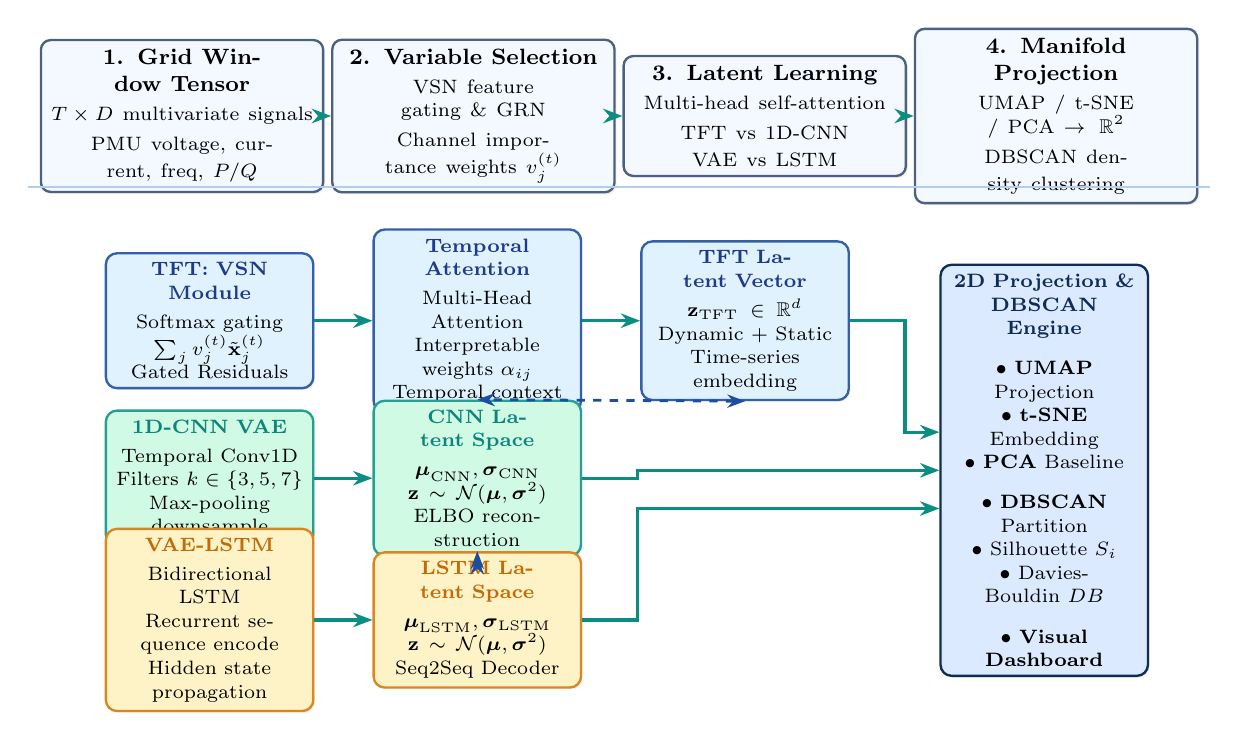
\begin{tikzpicture}[
  x=1cm, y=1cm,
  font=\sffamily,
  dagstep/.style={rectangle, rounded corners=3.5pt, minimum height=1.10cm,
    text width=3.35cm, align=center, draw=lavenderDark!75, fill=lavenderLight!75,
    line width=0.85pt, font=\fontsize{8.2}{9.8}\selectfont\bfseries,
    drop shadow={shadow xshift=0.8pt, shadow yshift=-0.8pt, opacity=0.10}},
  dagarrow/.style={-{Stealth[scale=0.85]}, line width=1.15pt, draw=prismTeal!95!black},
  blkbox/.style={rectangle, rounded corners=4pt, line width=0.85pt,
    minimum height=1.40cm, text width=2.40cm, align=center,
    font=\fontsize{7.2}{8.5}\selectfont, drop shadow={shadow xshift=0.6pt, shadow yshift=-0.6pt, opacity=0.12}},
  transbox/.style={rectangle, rounded corners=3pt, line width=0.80pt,
    draw=prismTeal!80, fill=cStage1!60, minimum height=1.15cm, text width=1.45cm, align=center,
    font=\fontsize{6.5}{7.6}\selectfont},
  skipconn/.style={-{Stealth[scale=0.75]}, line width=0.85pt, draw=prismNavy, dashed}
]

  % Row 1: 4-Stage Architectural Progression
  \node[dagstep] (s1) at (-5.55, 0) {1. Grid Window Tensor\\[2pt]\normalfont\fontsize{7.2}{8.5}\selectfont $T \times D$ multivariate signals\\[1pt]PMU voltage, current, freq, $P/Q$};
  \node[dagstep] (s2) at (-1.85, 0) {2. Variable Selection\\[2pt]\normalfont\fontsize{7.2}{8.5}\selectfont VSN feature gating \& GRN\\[1pt]Channel importance weights $v_j^{(t)}$};
  \node[dagstep] (s3) at (1.85, 0) {3. Latent Learning\\[2pt]\normalfont\fontsize{7.2}{8.5}\selectfont Multi-head self-attention\\[1pt]TFT vs 1D-CNN VAE vs LSTM};
  \node[dagstep] (s4) at (5.55, 0) {4. Manifold Projection\\[2pt]\normalfont\fontsize{7.2}{8.5}\selectfont UMAP / t-SNE / PCA $\to \mathbb{R}^2$\\[1pt]DBSCAN density clustering};

  \draw[dagarrow] (s1) -- (s2);
  \draw[dagarrow] (s2) -- (s3);
  \draw[dagarrow] (s3) -- (s4);

  % Separator
  \draw[draw=lavenderBorder, line width=0.6pt] (-7.5, -0.90) -- (7.5, -0.90);

  % Row 2 & 3: Detailed Architecture Branches
  % Branch 1: TFT (Primary)
  \node[blkbox, draw=prismBlue!90, fill=cStem] (b_tft_vsn) at (-5.20, -2.60) {
    \textbf{\color{prismIndigo}TFT: VSN Module}\\[2pt]
    Softmax gating\\
    $\sum_j v_j^{(t)} \tilde{\mathbf{x}}_j^{(t)}$\\
    Gated Residuals
  };

  \node[blkbox, draw=prismBlue!90, fill=cStem] (b_tft_attn) at (-1.80, -2.60) {
    \textbf{\color{prismIndigo}Temporal Attention}\\[2pt]
    Multi-Head Attention\\
    Interpretable weights $\alpha_{ij}$\\
    Temporal context
  };

  \node[blkbox, draw=prismBlue!90, fill=cStem] (b_tft_latent) at (1.60, -2.60) {
    \textbf{\color{prismIndigo}TFT Latent Vector}\\[2pt]
    $\mathbf{z}_{\text{TFT}} \in \mathbb{R}^d$\\
    Dynamic + Static\\
    Time-series embedding
  };

  \draw[dagarrow] (b_tft_vsn) -- (b_tft_attn);
  \draw[dagarrow] (b_tft_attn) -- (b_tft_latent);

  % Branch 2: 1D-CNN VAE (Baseline 1)
  \node[blkbox, draw=prismTeal!90, fill=cStage1] (b_cnn_vae) at (-5.20, -4.60) {
    \textbf{\color{prismTeal!90!black}1D-CNN VAE}\\[2pt]
    Temporal Conv1D\\
    Filters $k \in \{3, 5, 7\}$\\
    Max-pooling downsample
  };

  \node[blkbox, draw=prismTeal!90, fill=cStage1] (b_cnn_latent) at (-1.80, -4.60) {
    \textbf{\color{prismTeal!90!black}CNN Latent Space}\\[2pt]
    $\boldsymbol{\mu}_{\text{CNN}}, \boldsymbol{\sigma}_{\text{CNN}}$\\
    $\mathbf{z} \sim \mathcal{N}(\boldsymbol{\mu}, \boldsymbol{\sigma}^2)$\\
    ELBO reconstruction
  };

  \draw[dagarrow] (b_cnn_vae) -- (b_cnn_latent);

  % Branch 3: VAE-LSTM (Baseline 2)
  \node[blkbox, draw=prismGold!90, fill=cStage2] (b_lstm_vae) at (-5.20, -6.40) {
    \textbf{\color{prismGold!90!black}VAE-LSTM}\\[2pt]
    Bidirectional LSTM\\
    Recurrent sequence encode\\
    Hidden state propagation
  };

  \node[blkbox, draw=prismGold!90, fill=cStage2] (b_lstm_latent) at (-1.80, -6.40) {
    \textbf{\color{prismGold!90!black}LSTM Latent Space}\\[2pt]
    $\boldsymbol{\mu}_{\text{LSTM}}, \boldsymbol{\sigma}_{\text{LSTM}}$\\
    $\mathbf{z} \sim \mathcal{N}(\boldsymbol{\mu}, \boldsymbol{\sigma}^2)$\\
    Seq2Seq Decoder
  };

  \draw[dagarrow] (b_lstm_vae) -- (b_lstm_latent);

  % Unified Projection & Clustering Engine
  \node[blkbox, draw=lavenderDark, fill=cHead, minimum height=4.60cm, text width=2.40cm] (b_proj) at (5.40, -4.50) {
    \textbf{\color{lavenderDark}2D Projection \&}\\
    \textbf{\color{lavenderDark}DBSCAN Engine}\\[6pt]
    $\bullet$ \textbf{UMAP} Projection\\
    $\bullet$ \textbf{t-SNE} Embedding\\
    $\bullet$ \textbf{PCA} Baseline\\[6pt]
    $\bullet$ \textbf{DBSCAN} Partition\\
    $\bullet$ Silhouette $S_i$\\
    $\bullet$ Davies-Bouldin $DB$\\[6pt]
    $\bullet$ \textbf{Visual Dashboard}
  };

  % Convergence connections to Unified Engine
  \draw[dagarrow] (b_tft_latent.east) -- ++(0.7, 0) |- (b_proj.160);
  \draw[dagarrow] (b_cnn_latent.east) -- ++(0.7, 0) |- (b_proj.west);
  \draw[dagarrow] (b_lstm_latent.east) -- ++(0.7, 0) |- (b_proj.200);

  % Inter-model comparison link
  \draw[{Stealth[scale=0.85]}-{Stealth[scale=0.85]}, line width=1.0pt, dashed, draw=lavenderMedium]
    (b_tft_latent.south) -- (b_cnn_latent.north);
  \draw[{Stealth[scale=0.85]}-{Stealth[scale=0.85]}, line width=1.0pt, dashed, draw=lavenderMedium]
    (b_cnn_latent.south) -- (b_lstm_latent.north);

\end{tikzpicture}
\end{document}
